\documentclass[11pt]{article}
\usepackage[margin=1in]{geometry}
\usepackage{volfit_preamble}
\graphicspath{{figures/}}

\title{\textbf{Variance-Swap Targets}\\[2pt]
\large Log-contract replication, the LQD closed form, and the source-PDE method\\[2pt]
\normalsize Vol-Fitter Technical Notes, No.~08}
\author{Vol-Fitter}
\date{\today}

\begin{document}
\maketitle
% Auto-generated by gen_varswap.py — do not edit.
\newcommand{\vsclosed}{24.47}
\newcommand{\vsrepl}{24.49}
\newcommand{\vsagreebp}{1.53}
\newcommand{\vstarget}{25.97}
\newcommand{\vspulled}{25.91}
\newcommand{\vshalfwidth}{6.0}
\newcommand{\vspoints}{801}


\begin{abstract}
A variance-swap quote is one number per smile node --- the market's fair var-swap
volatility for an $(\text{underlying},T)$ --- and it pins a global property of the
smile that scattered option quotes constrain only weakly: the total risk-neutral
variance, dominated by the wings. This note documents how the Vol-Fitter turns a
var-swap quote into a soft calibration target shared by every model. The fair
var-swap total variance is the model-free OTM log-contract replication; the
penalty pulls the model's \emph{own} fair var-swap toward the quote, in vol units,
weighted as a chosen fraction of the node's option weight. Computing the model's
var-swap cheaply is the crux: the generic replication re-solves implied variance on
a grid every Jacobian column and would make a single fit take minutes, so LQD uses
its \emph{exact closed form} ($-2\,\E[X]$) and the local-vol surface uses a
\emph{source PDE} ($I(T)=g(0,1)$) with analytic sensitivities. A fresh run confirms
the LQD closed form agrees with replication to \vsagreebp\ vol bps, the replication
converges by a half-width of $\sim4$, and a var-swap quote $\vstarget\%$ pulls a
smile whose natural var-swap is $\vsclosed\%$ up to $\vspulled\%$ while keeping the
option fit.
\end{abstract}

\tableofcontents
\newpage

%======================================================================
\section{What a variance swap pins}
\label{sec:what}

A variance swap pays the realized variance of the underlying to $T$ against a
fixed strike. Under a diffusion the fair strike equals the risk-neutral expected
total variance, which the model-free Carr--Madan log-contract replication expresses
as a portfolio of OTM options:
\begin{equation}
w_{\text{vs}}(T)=\E^T\!\Big[\int_0^T\sigma_t^2\,\dd t\Big]
=2\!\int_0^\infty\frac{P(T,K)}{K^2}\dd K_{\text{put}}
+2\!\int^\infty\frac{C(T,K)}{K^2}\dd K_{\text{call}},
\label{eq:logcontract}
\end{equation}
the $1/K^2$ weighting placing most of the mass in the \emph{wings}. This is exactly
why a var-swap quote is informative: it constrains the total variance, a global
moment that a handful of near-the-money option quotes barely touch. A smile can fit
every quoted strike and still carry the wrong wing mass; the var-swap quote pins it.

\begin{heuristic}
Think of the var-swap as a single, very reliable ``wing quote''. Liquid options
cluster near the money, where they say little about the tails; the var-swap is a
traded instrument whose value is \emph{dominated} by the tails (the $1/K^2$
weight). Adding it to the objective is the cheapest way to discipline the
extrapolation the option quotes leave free --- complementary to the Lee wing
control of Note~09, which constrains the wing \emph{slope} while the var-swap
constrains the wing \emph{mass}.
\end{heuristic}

\begin{invariant}
\begin{enumerate}[leftmargin=1.6em]
\item One var-swap quote per node, model-independent, shared by the
parametric and local-vol views, with its own undo/redo history.
\item With no quote set (or the toggle off) every calibrator is
byte-identical to the un-targeted fit.
\item The model's own fair var-swap is computed by a route that is cheap
\emph{inside} the optimizer loop --- never by replication against a curve
that must be inverted per point.
\item The weight is relative (a fraction of the node's option weight), so
the target means the same thing on a 10-quote node and a 100-quote node.
\end{enumerate}
\end{invariant}

%======================================================================
\section{The replication and the penalty}
\label{sec:penalty}

In forward-normalized units ($F=1$, $k=\log K$), \eqref{eq:logcontract} becomes a
single integral over the normalized Black call $\Black(k,w(k))$,
\begin{equation}
w_{\text{vs}}=2\!\int_{-\infty}^{\infty}\!\Big[\Black(k,w(k))+(e^k-1)^-\Big]e^{-k}\,\dd k,
\label{eq:repl}
\end{equation}
evaluated by a trapezoid on $k\in[-H,H]$ with $H=\vshalfwidth$ and \vspoints\
points (the put leg adds $(e^k-1)e^{-k}$ for $k<0$). In code, \eqref{eq:repl} is a
trapezoid over any model's $w(k)$ (matches production to $10^{-9}$):

\begin{lstlisting}[caption={Model-free var-swap total variance by log-contract
replication \eqref{eq:repl} (distilled from \texttt{calib/varswap.py}).},
label={lst:repl}]
def varswap_total_variance(implied_w, half=6.0, n=801):   # implied_w(k) -> total variance
    k = np.linspace(-half, half, n)
    w = np.maximum(implied_w(k), 1e-12)
    integ = black_call(k, w)*np.exp(-k)              # OTM call leg, discounted
    put = k < 0
    integ[put] += 1 - np.exp(-k[put])               # (e^k - 1) e^{-k} on the put side
    return 2.0*np.trapezoid(integ, k)
\end{lstlisting}

The half-width is coarser than
the diagnostics grid because this runs \emph{inside} the optimizer loop; $\pm6$
captures the OTM mass to well under a basis point for any sane smile, as
\cref{fig:conv} confirms --- the fair var-swap vol has plateaued by a half-width of
$\sim4$.

The penalty is a single residual in \emph{volatility} units, so it stacks directly
onto the vol-space data residuals of SVI/SIV and the vega-normalized residuals of
LQD/LV:
\begin{equation}
\boxed{\;r_{\text{vs}}=\sqrt{\omega_{\text{vs}}}\,\big(\sigma_{\text{vs}}^{\text{model}}-\sigma_{\text{vs}}^{\text{quote}}\big),
\qquad \sigma_{\text{vs}}=\sqrt{w_{\text{vs}}/T}.\;}
\label{eq:vs_resid}
\end{equation}
The weight $\omega_{\text{vs}}$ is set to a chosen fraction (\texttt{varSwapWeightPct},
default $10\%$) of the node's summed option-quote weight, so the var-swap
contributes a controlled share of the total objective rather than an absolute,
scale-dependent amount.

\begin{figure}[H]
\centering
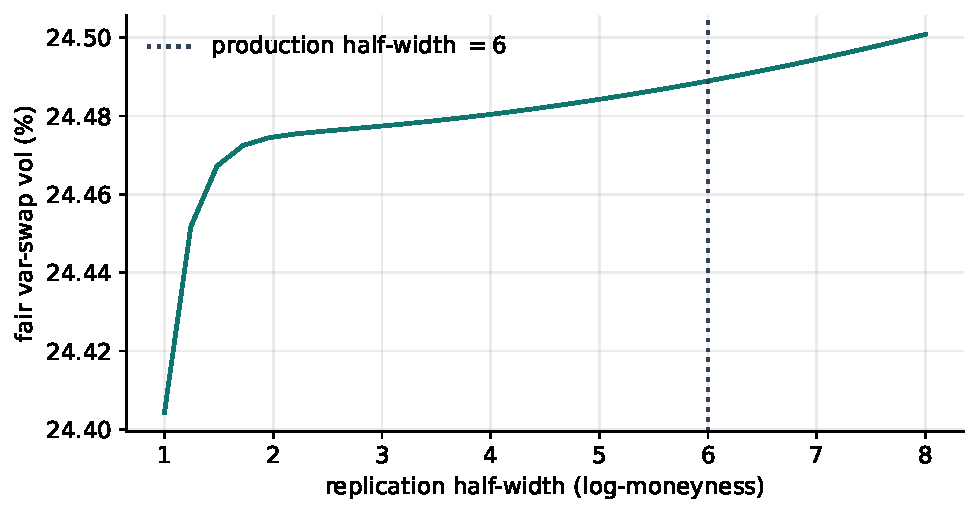
\includegraphics[width=0.70\textwidth]{fig_vs_convergence.pdf}
\caption{Fair var-swap volatility vs the replication half-width. The integral has
converged well before the production half-width of $6$.}
\label{fig:conv}
\end{figure}

%======================================================================
\section{Computing the model's var-swap cheaply}
\label{sec:cheap}

The penalty needs the \emph{model's} fair var-swap at every optimizer iteration.

\begin{example}[title={Case file: the fit that took minutes}]
\textbf{Setup.} The first wiring of the var-swap penalty used the generic
replication \eqref{eq:repl} for every model --- correct, uniform, and
obviously fine, since the integral is just a trapezoid.

\textbf{Failure mode.} LQD fits with a var-swap target went from milliseconds
to \emph{minutes}, hanging the calibrate loop.

\textbf{Diagnosis.} The replication calls the model's
$\texttt{implied\_w}(k)$ on $\sim800$ points --- and for LQD each point is a
Black \emph{inversion} of a quadrature-priced call. Inside a
finite-difference Jacobian that is $\sim800$ root-finds \emph{per parameter
column per iteration}: thousands of inversions to price one number the model
knows in closed form.

\textbf{Fix.} Per-model routes (below): LQD prices the log contract exactly
as $-2\,\E[X]$ on its existing grid; SVI/SIV keep the replication because
their $w(k)$ is arithmetic (evaluated, never solved); the LV surface gets a
source PDE with analytic sensitivities.

\textbf{Verdict.} The closed form agrees with the replication to
\vsagreebp\ vol bps (validating both), and the var-swap penalty now costs
essentially nothing in any model. The lesson generalizes: \emph{a uniform
implementation is not a virtue when the models' native objects differ ---
route each model through what it already computes.}
\end{example}

\subsection{LQD: the exact closed form}

For LQD the var-swap is a one-line consequence of the log-contract identity
$\E[-2X]=-2\int_0^1 Q(u)\,\dd u$. In the logit coordinate this is a single
quadrature against the \emph{same} grid the slice already built,
\begin{equation}
w_{\text{vs}}^{\text{LQD}}=-2\,\E[X]=-2\!\int_{-\infty}^{\infty}Q(z)\,\Lambda(z)(1-\Lambda(z))\,\dd z,
\label{eq:lqd_vs}
\end{equation}
whose integrand decays like $z\,e^{-|z|}$. No inversion, no extra grid --- it is
essentially free. \Cref{tab:vs} confirms it agrees with the generic replication to
\vsagreebp\ vol bps, validating both.

\subsection{SVI and SIV: arithmetic curves}

For SVI and Multi-Core SIV the total variance $w(k)$ is closed-form arithmetic
(a hyperbola, or a log-cosh sum), so the replication \eqref{eq:repl} is cheap
directly --- no inversion is needed because $w(k)$ is evaluated, not solved.

\subsection{Local volatility: the source PDE}

The piecewise-affine surface has no arithmetic $w(k)$; pricing each $k$ means a PDE
solve. The \emph{source-PDE} method (Note~04) instead reads the var-swap off one
backward parabolic solve,
\begin{equation}
\partial_t g+\tfrac12\nu(t,x)x^2\partial_{xx}g+\nu=0,\quad g(T,\cdot)=0,
\qquad I(T)=g(0,1),
\label{eq:source_pde}
\end{equation}
with analytic sensitivities $\partial I/\partial\theta$ from the same multi-RHS
machinery as the value solve, and --- unlike the replication --- no dependence on
the truncation $x_{\max}$. It is gated by \texttt{varSwapMethod} (default
\texttt{static} replication; the source PDE is the faster alternative).

%======================================================================
\section{Worked example}
\label{sec:example}

\Cref{fig:fit} fits an LQD slice to an index-like smile whose \emph{natural} fair
var-swap is $\vsclosed\%$, then refits it with a var-swap quote of $\vstarget\%$
($1.5$ vol points higher) at $10\%$-class weight. The targeted fit lifts its fair
var-swap to $\vspulled\%$ --- almost all the way to the quote --- while still
threading the option quotes: the var-swap adds wing mass the near-the-money options
did not constrain. \Cref{tab:vs} collects the numbers.

\begin{figure}[H]
\centering
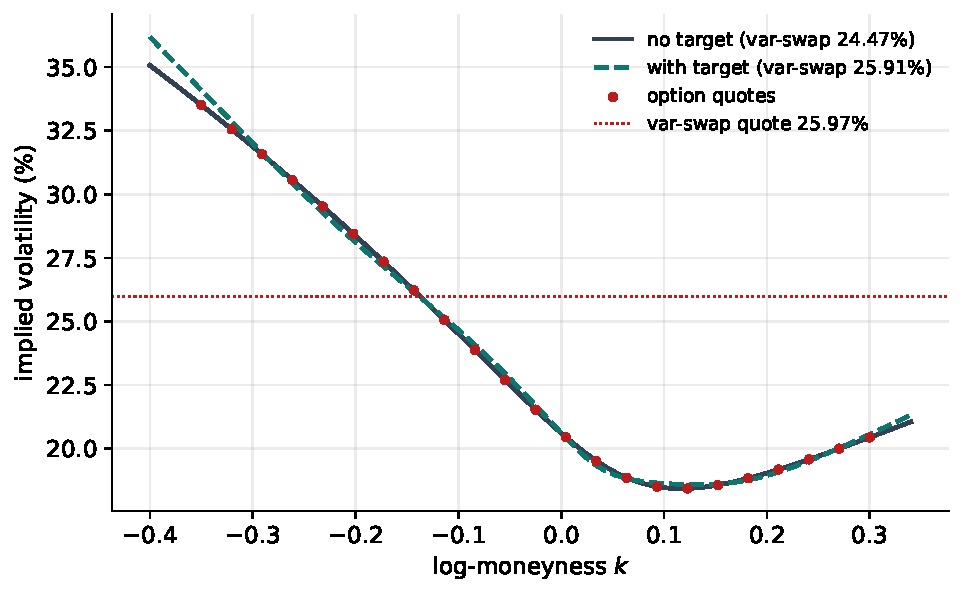
\includegraphics[width=0.80\textwidth]{fig_vs_fit.pdf}
\caption{An LQD fit with (dashed) and without (solid) a var-swap target above the
smile's natural level. The target lifts the fair var-swap toward the quote by
adding wing mass while keeping the option fit.}
\label{fig:fit}
\end{figure}

\begin{table}[H]
\centering
\caption{Var-swap numbers (fresh run): closed form vs replication, and the
targeted pull.}
\label{tab:vs}
\begin{tabular}{lr}
\toprule
Quantity & Value\\
\midrule
LQD closed-form var-swap vol & $\vsclosed\%$\\
Replication var-swap vol & $\vsrepl\%$\\
Closed-form vs replication agreement & $\vsagreebp$ vol bp\\
Var-swap quote (target) & $\vstarget\%$\\
Targeted-fit fair var-swap & $\vspulled\%$\\
\bottomrule
\end{tabular}
\end{table}

%======================================================================
\section{What is original here}
\label{sec:original}

The log-contract replication is Carr--Madan; the contributions are practical. The
\emph{per-model cheap var-swap} --- LQD's closed form \eqref{eq:lqd_vs}, SVI/SIV's
arithmetic curves, and the LV source PDE \eqref{eq:source_pde} with analytic
sensitivities --- is what makes a var-swap target affordable \emph{inside} the
optimizer loop rather than as a slow post-hoc check; and the \emph{relative}
weighting (a fraction of the node's option weight) keeps the target scale-free
across nodes with very different quote counts. Together they make one extra global
constraint cost essentially nothing.

%======================================================================
\section{Traceability}
\label{sec:traceability}

\begingroup
\small
\setlength{\tabcolsep}{3pt}
\begin{longtable}{@{}p{0.32\textwidth}p{0.11\textwidth}p{0.24\textwidth}p{0.29\textwidth}@{}}
\caption{Claims in this note and the code/tests that lock them.}\\
\toprule Claim & Object & Code anchor & Test anchor\\ \midrule
\endfirsthead
\toprule Claim & Object & Code anchor & Test anchor\\ \midrule
\endhead
Penalty pulls every model toward the quote &
\eqref{eq:vs_resid} &
\nolinkurl{calib/varswap.py} &
\nolinkurl{test_varswap.py::test_penalty_pulls_model_varswap_toward_quote_all_models}\\
No target / disabled is byte-identical &
invariant~2 &
\nolinkurl{calib/varswap.py} &
\nolinkurl{test_varswap.py::test_none_target_is_byte_identical}, \nolinkurl{::test_disabling_varswap_drops_the_penalty}\\
Weight strength monotone &
\eqref{eq:vs_resid} &
\nolinkurl{calib/varswap.py} &
\nolinkurl{test_varswap.py::test_weight_strength_monotone}\\
Session set/exclude/undo/redo &
invariant~1 &
\nolinkurl{api/varswap_session.py} &
\nolinkurl{test_varswap.py::test_session_set_exclude_include_remove}, \nolinkurl{::test_session_undo_redo_and_validation}\\
LV fit carries and honours the quote &
\cref{sec:cheap} &
\nolinkurl{api/affine_fit.py} &
\nolinkurl{test_varswap.py::test_affine_fit_carries_and_honours_varswap}\\
Source PDE matches static; analytic sensitivities &
\eqref{eq:source_pde} &
\nolinkurl{models/localvol/varswap_pde.py} &
\nolinkurl{test_varswap_source.py::test_source_pde_value_matches_static}, \nolinkurl{::test_source_pde_theta_sensitivity_matches_fd}\\
LQD closed form (the case-file fix) &
\eqref{eq:lqd_vs} &
\nolinkurl{models/lqd/quadrature.py::var_swap_strike} &
\nolinkurl{test_varswap.py} (all-models pull), agreement figure \vsagreebp\ bp\\
\bottomrule
\end{longtable}
\endgroup

\appendix
%======================================================================
\section{Hyperparameter atlas}
\label{app:atlas}

\begin{longtable}{p{0.26\textwidth}p{0.14\textwidth}p{0.52\textwidth}}
\caption{Variance-swap hyperparameters.}\label{tab:atlas}\\
\toprule Knob & Default & Role\\ \midrule
\endfirsthead \toprule Knob & Default & Role\\ \midrule \endhead
\multicolumn{3}{l}{\emph{Surfaced}}\\ \midrule
\texttt{varSwapEnabled} & \texttt{true} & Master toggle (surfaces the var-swap
level); the penalty itself activates only when a quote is set on the node.\\
\texttt{varSwapWeightPct} & $10\%$ & Var-swap weight as a fraction of node option weight.\\
\texttt{varSwapMethod} (LV) & \texttt{static} & Replication or source-PDE pricer.\\
\midrule
\multicolumn{3}{l}{\emph{Hidden}}\\ \midrule
\texttt{VS\_HALF\_WIDTH} $H$ & $\vshalfwidth$ & Replication half-width in log-moneyness.\\
\texttt{VS\_POINTS} & $\vspoints$ & Replication trapezoid points.\\
\texttt{\_W\_FLOOR} & $10^{-12}$ & Total-variance floor in the integrand.\\
\bottomrule
\end{longtable}

\noindent\textbf{Performance.} The LQD closed form is one quadrature on the
existing grid (free); the replication is $\sim800$ arithmetic evaluations for
SVI/SIV (negligible); the LV source PDE is one extra backward solve with analytic
sensitivities. Using the generic replication on an LQD curve --- $\sim800$ Black
inversions per Jacobian column --- would turn a millisecond fit into minutes, which
is the whole reason for the per-model routes of \cref{sec:cheap}.

%======================================================================
\section{Reference implementation: the LQD closed form}
\label{app:ref}

For LQD the fair var-swap total variance is $-2\,\E[X]$ with no replication integral
and no Black inversions: the log contract is exactly the mean log-return, and the
quadrature grid already carries $Q(z)$ and $u(1-u)$ (Note~01). Agrees with the
generic replication to \vsagreebp\ vol bps and with production to $10^{-12}$.

\begin{lstlisting}[caption={The LQD closed-form var-swap strike, the mean
log-return (distilled from \texttt{models/lqd/quadrature.py}).}]
def var_swap_strike(z, q_z, u):           # z: logit grid, q_z = Q(z), u = expit(z)
    return -2.0 * np.trapezoid(q_z * u * (1 - u), z)   # = -2 E[X], the log contract
\end{lstlisting}

\begin{thebibliography}{9}
\bibitem{CarrMadan1998} P.~Carr and D.~Madan. Towards a theory of volatility
trading. In \emph{Volatility}, Risk Books, 1998.
\bibitem{DemeterfiDermanKamalZou1999} K.~Demeterfi, E.~Derman, M.~Kamal and J.~Zou.
A guide to volatility and variance swaps. \emph{J.\ Derivatives}, 6(4):9--32, 1999.
\bibitem{Gatheral2006} J.~Gatheral. \emph{The Volatility Surface}. Wiley, 2006.
\end{thebibliography}

\end{document}
